\documentclass{beamer}
\usepackage{tikz}
\usetikzlibrary{matrix}
\begin{document}


\begin{frame}{Sign Domain}
\begin{tikzpicture}[baseline]every node/.style={anchor=base,text depth=.5ex,text height=2ex,text width=1em}
\matrix (a) [matrix of math nodes, column sep=0.2cm, row sep=0.2cm, ampersand replacement=\&]{
\&\top\&\\
+\&0\& -\\
\&\bot\&\\};

\foreach \i/\j in {1-2/2-1, 1-2/2-2, 1-2/2-3,%
            3-2/2-1, 3-2/2-2, 3-2/2-3%
            }
    \draw (a-\i) -- (a-\j);

\end{tikzpicture} $\langle Sign,\sqsubseteq\rangle$ \hfill $\begin{array}{l}\alpha_{sign}: \wp(Z)\mapsto Sign \\
\gamma_{sign}: Sign \mapsto \wp(Z) 
 \end{array}$
 
\begin{eqnarray*}
\alpha_{sign}(X) &=& \left\{\begin{array}{ll} 
                +  & \mbox{if $X\subseteq\{n | n > 0\}$}\\
                0  & \mbox{if $X=\{0\}$}\\
                -  & \mbox{if $X\subseteq\{n | n < 0\}$}\\
                \bot & \mbox{if $X=\emptyset$}\\
                \top  & \mbox{otherwise}\\
        \end{array}\right.\\
\gamma_{sign}(s)  &=& \left\{\begin{array}{ll} \{ n | n > 0\} & \mbox{if $s=+$} \\
                                \{0\} & \mbox{if $s=0$} \\
                                \{ n | n < 0\} & \mbox{if $s=-$} \\
                                Z & \mbox{if $s=\top$} \\
                                \emptyset & \mbox{if $s=\bot$} \\
                            \end{array}\right.
\end{eqnarray*}
\end{frame}

\begin{frame}{Disjunctive Completion} 
The idea of disjunctive completion is to construct a more precise abstract domain from an existing abstract domain such that
\begin{itemize}[<+->]
\item the least upper bound operation is preserved by the concretization function
\item the concretization function commutes with the least upper bound operation
\item This takes a number of steps
\begin{itemize}
\item Apply the power set construction  to the existing domain. 
      \begin{eqnarray*} \gamma_{sign}^* &: & \wp(Sign) \mapsto \wp(Z) \\ 
            \gamma_{sign}^* (S) &= & \bigcup \{ \gamma_{sign}(s) \mid s\in S\} 
      \end{eqnarray*}  
\item Remove redundant elements from the power set.
\item Simplify the representation of the resulting domain. 
\end{itemize}
\end{itemize}
\end{frame}




\begin{frame}{Disjunction Completion of Sign}

\hfill 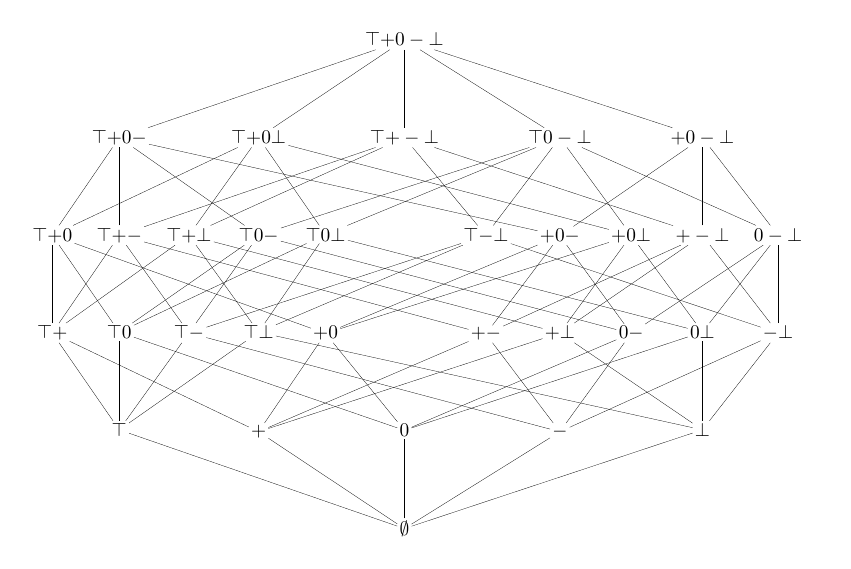
\begin{tikzpicture}[remember picture,
%overlay,
every node/.style={%anchor=base, %text depth=.5ex,text height=2ex,text width=1em,
    inner sep =1pt, scale = 0.7
    }
]
\matrix (c) [matrix of math nodes, column sep=0.2cm, row sep=1cm, ampersand replacement=\&]{
\&\&\&\&\&\top{+}0-\bot \&\&\&\&\&\\
 \& \top{+}0- \&\& \top{+}0\bot\&\& \top{+}-\bot\&\& \top{0}-\bot\&\& +0-\bot \&\\
\top{+}0 \& \top{+}- \& \top{+}\bot\& \top{0}-\& \top{0}\bot\&\& \top{-}\bot\& +0-\& +0\bot\& +-\bot\& 0-\bot \\
\top{+}\& \top{0}\& \top{-}\& \top\bot\& +0\&\& +-\& +\bot\& 0-\& 0\bot\& -\bot \& \\
 \& \top \&\& + \&\& 0 \&\& - \&\& \bot \& \\
\&\&\&\&\&\emptyset \&\&\&\&\&\\
};

\foreach \i/\j in {5-2/4-1, 5-2/4-2, 5-2/4-3,5-2/4-4,%
                   5-4/4-1, 5-4/4-5, 5-4/4-7,5-4/4-8,%
                   5-6/4-2, 5-6/4-5, 5-6/4-9,5-6/4-10,%
                   5-8/4-3, 5-8/4-7, 5-8/4-9,5-8/4-11,%
                   5-10/4-4, 5-10/4-8, 5-10/4-10,5-10/4-11,%
                   4-1/3-1, 4-1/3-2, 4-1/3-3,
                   4-2/3-1, 4-2/3-4, 4-2/3-5,
                   4-3/3-2, 4-3/3-4, 4-3/3-7,
                   4-4/3-3, 4-4/3-5, 4-4/3-7,
                   4-5/3-1, 4-5/3-8, 4-5/3-9,
                   4-7/3-2, 4-7/3-8, 4-7/3-10,
                   4-8/3-3, 4-8/3-9, 4-8/3-10,
                   4-9/3-4, 4-9/3-8, 4-9/3-11,
                   4-10/3-5, 4-10/3-9, 4-10/3-11,
                   4-11/3-7, 4-11/3-10, 4-11/3-11,
                   3-1/2-2, 3-1/2-4,
                   3-2/2-2, 3-2/2-6,
                   3-3/2-4, 3-3/2-6,
                   3-4/2-2, 3-4/2-8,
                   3-5/2-4, 3-5/2-8,%
                   3-7/2-6, 3-7/2-8,
                   3-8/2-2, 3-8/2-10,
                   3-9/2-4, 3-9/2-8,
                   3-10/2-6, 3-10/2-10,
                   3-11/2-8, 3-11/2-10,
                   6-6/5-2,  6-6/5-4, 6-6/5-6, 6-6/5-8, 6-6/5-10,
                   1-6/2-2,  1-6/2-4, 1-6/2-6, 1-6/2-8, 1-6/2-10%
            }
    \draw [line width=0.1pt] (c-\i) -- (c-\j);


\end{tikzpicture}

\begin{tikzpicture}[remember picture,overlay]
\draw<2->[draw=blue,thin]
(c-5-2.south west) -- (c-5-2.south east)  --
(c-4-4.south east) -- (c-4-4.north east)--
(c-3-7.south east) -- (c-3-7.north east) --
(c-2-8.south east) -- (c-2-8.north east) --
(c-1-6.north east) -- (c-1-6.north west)
-- (c-2-2.north west) -- (c-2-2.south west) -- (c-3-1.north west) -- (c-3-1.south west) -- (c-4-1.south west) -- cycle
;
\end{tikzpicture}

\begin{overlayarea}{\textwidth}{2.5cm}
\only<2>{\small All these elements have the same meaning - their images under $\gamma_{sign}^*$ are the same. 
For any set of signs S, $\gamma_{sign}^*(S) = \gamma_{sign}^*(\downarrow S)$. 
\[ \downarrow S = \{s' | \exists s\in S. (s'\sqsubseteq s)\}
\]}
\end{overlayarea}
\end{frame}

\begin{frame}

\hfill 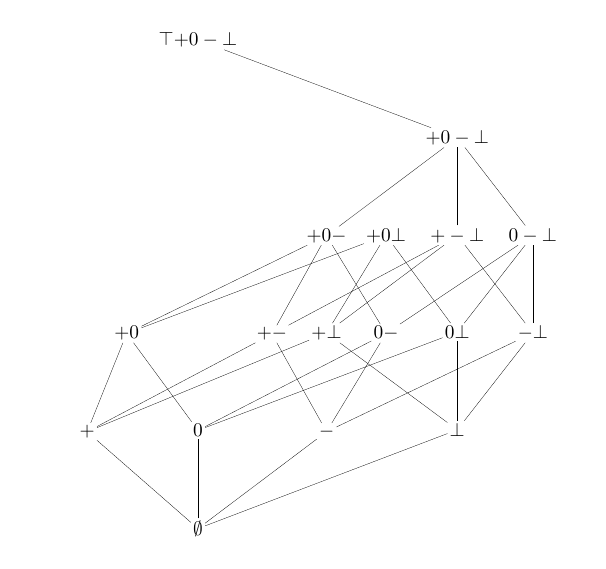
\begin{tikzpicture}[remember picture,
%overlay,
every node/.style={%anchor=base, %text depth=.5ex,text height=2ex,text width=1em,
    inner sep =1pt, scale = 0.7
    }
]
\matrix (c) [matrix of math nodes, column sep=0.2cm, row sep=1cm, ampersand replacement=\&]{
\&\&\&\&\&\top{+}0-\bot \&\&\&\&\&\\
 \&  \&\& \&\& \&\& \&\& +0-\bot \&\\
\& \& \& \& \&\& \& +0-\& +0\bot\& +-\bot\& 0-\bot \\
\& \& \& \& +0\&\& +-\& +\bot\& 0-\& 0\bot\& -\bot \& \\
 \& \&\& + \&\& 0 \&\& - \&\& \bot \& \\
\&\&\&\&\&\emptyset \&\&\&\&\&\\
};

\foreach \i/\j in {
                   5-4/4-5, 5-4/4-7,5-4/4-8,%
                   5-6/4-5, 5-6/4-9,5-6/4-10,%
                    5-8/4-7, 5-8/4-9,5-8/4-11,%
                    5-10/4-8, 5-10/4-10,5-10/4-11,%
                          4-5/3-8, 4-5/3-9,
                   4-7/3-8, 4-7/3-10,
                    4-8/3-9, 4-8/3-10,
                    4-9/3-8, 4-9/3-11,
                    4-10/3-9, 4-10/3-11,
                  4-11/3-10, 4-11/3-11,
                    3-8/2-10,
                    3-10/2-10,
                   3-11/2-10,
                  6-6/5-4, 6-6/5-6, 6-6/5-8, 6-6/5-10,
                   1-6/2-10%
            }
    \draw [line width=0.1pt] (c-\i) -- (c-\j);


\end{tikzpicture}

\begin{tikzpicture}[remember picture,overlay]

\draw<2>[draw=green,thin] (c-3-8.south west) rectangle (c-3-8.north east);
\draw<2>[draw=green,thin] (c-2-10.south west) rectangle (c-2-10.north east);
\draw<2>[draw=green,thick] (c-3-8.north east) -- (c-2-10.south west);

\draw<2>[draw=red,thin] (c-3-9.south west) rectangle (c-3-9.north east);
\draw<2>[draw=red,thin] (c-4-5.south west) rectangle (c-4-5.north east);
\draw<2>[draw=red,thick] (c-3-9.south west) -- (c-4-5.north east);



\draw<2>[draw=black,thin] (c-3-10.south west) rectangle (c-3-10.north east);
\draw<2>[draw=black,thin] (c-4-7.south west) rectangle (c-4-7.north east);
\draw<2>[draw=black,thick] (c-3-10.south west) -- (c-4-7.north east);

\draw<2>[draw=purple,thin] (c-3-11.south west) rectangle (c-3-11.north east);
\draw<2>[draw=purple,thin] (c-4-9.south west) rectangle (c-4-9.north east);
\draw<2>[draw=purple,thick] (c-3-11.south west) -- (c-4-9.north east);

\end{tikzpicture}
\end{frame}


\begin{frame}

\hfill \begin{tikzpicture}[remember picture,
%overlay,
every node/.style={%anchor=base, %text depth=.5ex,text height=2ex,text width=1em,
    inner sep =1pt, scale = 0.7
    }
]
\matrix (c) [matrix of math nodes, column sep=0.2cm, row sep=1cm, ampersand replacement=\&]{
\&\&\&\&\&\top{+}0-\bot \&\&\&\&\&\\
 \&  \&\& \&\& \&\& \&\& +0-\bot \&\\
\& \& \& \& \&\& \& \& +0\bot\& +-\bot\& 0-\bot \\
\& \& \& \& \&\& \& +\bot\& \& 0\bot\& -\bot \& \\
 \& \&\& + \&\& 0 \&\& - \&\& \bot \& \\
\&\&\&\&\&\emptyset \&\&\&\&\&\\
};

\foreach \i/\j in {
                  5-4/4-8,%
                   5-6/4-10,%
                    5-8/4-11,%
                    5-10/4-8, 5-10/4-10,5-10/4-11,%
                      4-8/3-9, 4-8/3-10,
                      4-10/3-9, 4-10/3-11,
                  4-11/3-10, 4-11/3-11,
                    3-9/2-10,
                    3-10/2-10,
                   3-11/2-10,
                  6-6/5-4, 6-6/5-6, 6-6/5-8, 6-6/5-10,
                   1-6/2-10%
            }
    \draw [line width=0.1pt] (c-\i) -- (c-\j);


\end{tikzpicture}

\begin{tikzpicture}[remember picture,overlay]

\draw<2>[draw=red,thin] (c-4-11.south west) rectangle (c-4-11.north east);
\draw<2>[draw=red,thin] (c-5-8.south west) rectangle (c-5-8.north east);
\draw<2>[draw=red,thick] (c-4-11.south west) -- (c-5-8.north east);



\draw<2>[draw=black,thin] (c-4-10.south west) rectangle (c-4-10.north east);
\draw<2>[draw=black,thin] (c-5-6.south west) rectangle (c-5-6.north east);
\draw<2>[draw=black,thick] (c-4-10.south west) -- (c-5-6.north east);

\draw<2>[draw=purple,thin] (c-5-4.south west) rectangle (c-5-4.north east);
\draw<2>[draw=purple,thin] (c-4-8.south west) rectangle (c-4-8.north east);
\draw<2>[draw=purple,thick] (c-4-8.south west) -- (c-5-4.north east);

\end{tikzpicture}
\end{frame}

\begin{frame}

\hfill \begin{tikzpicture}[remember picture,
%overlay,
every node/.style={%anchor=base, %text depth=.5ex,text height=2ex,text width=1em,
    inner sep =1pt, scale = 0.7
    }
]
\matrix (c) [matrix of math nodes, column sep=0.2cm, row sep=1cm, ampersand replacement=\&]{
\&\&\&\&\&\top{+}0-\bot \&\&\&\&\&\\
 \&  \&\& \&\& \&\& \&\& +0-\bot \&\\
\& \& \& \& \&\& \& \& +0\bot\& +-\bot\& 0-\bot \\
\& \& \& \& \&\& \& +\bot\& \& 0\bot\& -\bot \& \\
 \& \&\& \&\&  \&\&  \&\& \bot \& \\
\&\&\&\&\&\emptyset \&\&\&\&\&\\
};

\foreach \i/\j in {
                    5-10/4-8, 5-10/4-10,5-10/4-11,%
                      4-8/3-9, 4-8/3-10,
                      4-10/3-9, 4-10/3-11,
                  4-11/3-10, 4-11/3-11,
                    3-9/2-10,
                    3-10/2-10,
                   3-11/2-10,
                  6-6/5-10,
                   1-6/2-10%
            }
    \draw [line width=0.1pt] (c-\i) -- (c-\j);


\end{tikzpicture}

\begin{tikzpicture}[remember picture,overlay]
\draw<2>[draw=black,thin] (c-2-10.south west) rectangle (c-2-10.north east);
\draw<2>[draw=black,thin] (c-1-6.south west) rectangle (c-1-6.north east);
\draw<2>[draw=black,thick] (c-2-10.north west) -- (c-1-6.south east);

\draw<2>[draw=red,thin] (c-5-10.south west) rectangle (c-5-10.north east);
\draw<2>[draw=red,thin] (c-6-6.south west) rectangle (c-6-6.north east);
\draw<2>[draw=red,thick] (c-5-10.south west) -- (c-6-6.north east);
\end{tikzpicture}
\end{frame}

\begin{frame}

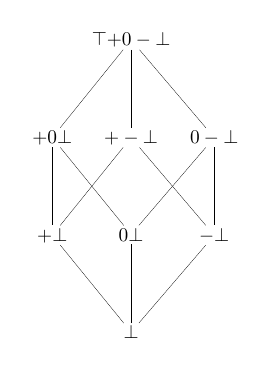
\begin{tikzpicture}[
every node/.style={%anchor=base, %text depth=.5ex,text height=2ex,text width=1em,
    inner sep =1pt, scale = 0.7
    }
]
\matrix (c) [matrix of math nodes, column sep=0.2cm, row sep=1cm, ampersand replacement=\&]{
\&\top{+}0-\bot \&\\
+0\bot\& +-\bot\& 0-\bot \\
+\bot\&  0\bot\& -\bot  \\
\& \bot \& \\
};

\foreach \i/\j in { 1-2/2-1,1-2/2-2,1-2/2-3,
                    4-2/3-1,4-2/3-2,4-2/3-3,
                    2-1/3-1,2-1/3-2,
                    2-2/3-1,2-2/3-3,
                    2-3/3-2,2-3/3-3%
            }
    \draw [line width=0.1pt] (c-\i) -- (c-\j);
\end{tikzpicture} \hfill
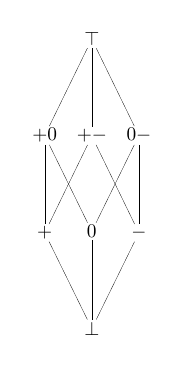
\begin{tikzpicture}[
every node/.style={%anchor=base, %text depth=.5ex,text height=2ex,text width=1em,
    inner sep =1pt, scale = 0.7
    }
]
\matrix (c) [matrix of math nodes, column sep=0.2cm, row sep=1cm, ampersand replacement=\&]{
\&\top \&\\
+0 \& +- \& 0- \\
+\&  0\& -  \\
\& \bot \& \\
};

\foreach \i/\j in { 1-2/2-1,1-2/2-2,1-2/2-3,
                    4-2/3-1,4-2/3-2,4-2/3-3,
                    2-1/3-1,2-1/3-2,
                    2-2/3-1,2-2/3-3,
                    2-3/3-2,2-3/3-3%
            }
    \draw [line width=0.1pt] (c-\i) -- (c-\j);
\end{tikzpicture}


\end{frame}

\begin{frame}{Disjunctive Completion} 
Given an abstract domain $\langle A, \sqsubseteq_A\rangle$ with $\langle \alpha,\gamma\rangle$, construct 
\begin{itemize}
    \item $\langle A^\vee, \subseteq_A\rangle$ where 
    	\[A^\vee = \{X \subseteq A \mid X = \downarrow X\} \] 
    \item Identify elements on $A^\vee$ with the same meaning under $\gamma^*$. 
    \item The Galois connection is then defined as 
    \begin{eqnarray*}
    \gamma^\vee(X) &=& \bigcup\{\gamma(a) \mid a\in X\}\\
    \alpha^\vee(c) &=& \bigcap \{ X \mid c\sqsubseteq_C \gamma^\vee(X)\} 
    \end{eqnarray*}    	
\end{itemize}
\end{frame}

\end{document} 

\begin{tikzpicture}every node/.style={anchor=base,text depth=.5ex,text height=2ex,text width=1em}

\matrix (a) [matrix of math nodes, column sep=0.2cm, row sep=0.2cm, ampersand replacement=\&]{
\&\top\&\\
+\&0\& -\\
\&\bot\&\\};

\foreach \i/\j in {1-2/2-1, 1-2/2-2, 1-2/2-3,%
            3-2/2-1, 3-2/2-2, 3-2/2-3%
            }
    \draw (a-\i) -- (a-\j);

\end{tikzpicture}


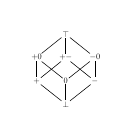
\begin{tikzpicture}[
every node/.style={anchor=base, %text depth=.5ex,text height=2ex,text width=1em,
    inner sep =1pt, scale = 0.3}
]
\matrix (b) [matrix of math nodes, column sep=0.2cm, row sep=0.2cm, ampersand replacement=\&
]{\scriptscriptstyle
\&\top\&\\
+0 \& +- \& -0\\
+\&0\& -\\
\&\bot\&\\};

\foreach \i/\j in {1-2/2-1, 1-2/2-2, 1-2/2-3,%
                   2-1/3-1, 2-1/3-2, 2-2/3-1, 2-2/3-3, 2-3/3-2, 2-3/3-3,%
                   4-2/3-1, 4-2/3-2, 4-2/3-3%
            }
    \draw [line width=0.2pt] (b-\i) -- (b-\j);

%\draw[double,densely dotted] (a-2-2)--(a-3-2) (a-2-4)--(a-3-4);
\end{tikzpicture}


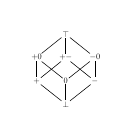
\begin{tikzpicture}[
every node/.style={anchor=base, %text depth=.5ex,text height=2ex,text width=1em,
    inner sep =1pt, scale = 0.3}
]
\matrix (d) [matrix of math nodes, column sep=0.2cm, row sep=0.2cm, ampersand replacement=\&
]{%\scriptscriptstyle
\&\top\&\\
+0 \& +- \& -0\\
+\&0\& -\\
\&\bot\&\\};

\foreach \i/\j in {1-2/2-1, 1-2/2-2, 1-2/2-3,%
                   2-1/3-1, 2-1/3-2, 2-2/3-1, 2-2/3-3, 2-3/3-2, 2-3/3-3,%
                   4-2/3-1, 4-2/3-2, 4-2/3-3%
            }
    \draw [line width=0.2pt] (d-\i) -- (d-\j);

%\draw[double,densely dotted] (a-2-2)--(a-3-2) (a-2-4)--(a-3-4);
\end{tikzpicture}

\end{frame}